\section{Conformance Test Cases for the RDF Mapping Language}

%Knowledge graphs are often generated based on rules that apply semantic annotations to certain data. For example, the DBpedia knowledge graph is generated by applying classes and predicates of the DBpedia ontology to Wikipedia \citep{lehmann_2015_swj}. Software tools execute these rules and generate corresponding RDF triples and quads \citep{RDF}, which materialize knowledge graphs. In the past, custom scripts prevailed, but lately rule-driven tools emerged. Such tools distinguish the rules that define how RDF terms and triples are generated from the tool that executes them. R2RML \citep{R2RML} is the W3C recommended language to define such rules for generating knowledge graphs from data in relational databases (RDBs). An R2RML processor is a system that, given a set of R2RML rules and a relational database, generates an output RDF dataset. Examples of R2RML processors are, e.g., Ultrawrap \citep{sequeda_2013_jws}, Morph-RDB \citep{priyatna2014formalisation}, Ontop \citep{calvanese2017ontop}, and XSPARQL \citep{bischof_2012_jds}. A subset of them was included in the RDB2RDF Implementation Report \citep{R2RML} to determine their conformance to the R2RML specification \footnote{Some of those available in the report are no longer actively maintained and used}, i.e., the correct knowledge graph is generated for a set of rules and certain relational database.

%Need: Why something needed to be done at all
%Extensions and adaptations were applied to R2RML to account for other types of data sources, given that R2RML is focused on relational databases only, such as RML~\citep{dimou2014rml}, XSPARQL~\citep{bischof_2012_jds}, xR2RML~\citep{michel2015translation}, KR2RML~\citep{slepicka2015kr2rml}, and D2RML~\citep{chortaras2018d2rml}. RML provides an extension of R2RML to support heterogeneous data sources, including different formats, e.g., CSV, XML, JSON, and access interfaces, e.g., files and Web APIs. Similarly, RML processors emerged that execute RML rules, such as the RMLMapper\footnote{RMLMapper, \url{https://github.com/RMLio/rmlmapper-java}}, CARML\footnote{CARML, \url{https://github.com/carml/carml}}, GeoTriples\footnote{GeoTriples, \url{https://github.com/LinkedEOData/GeoTriples}}, and Ontario\footnote{Ontario,\url{https://github.com/WDAqua/Ontario}}.
Unlike R2RML, there are no test cases available to determine the conformance of the processors to the RML specification. As a result, the processors are either not tested or only tested with custom test cases, which do not necessarily assess every aspect of the specification. Consequently, no implementation report is available that allows comparing the different processors that generate knowledge graphs from heterogeneous data sources
based on the conformance to the specification. This way it is hard to determine the most suitable processor for a certain use case.

%Task: What was undertaken to address the need
%Object: What the present document does or covers
In this section, we focused on RML and introduce an initial set of RML test cases, which contains 297 test cases based on the existing R2RML test cases. However, instead of only considering relational databases as data sources, as it occurs for the R2RML test cases, we also consider data in CSV, XML, and JSON format. Furthermore, we tested the conformance of the RMLMapper, RocketRML, SDM-RDFizer and CARML: every test case is executed by each processor and we noted if the generated knowledge graph matches the expected one. The corresponding implementation report is available at \url{http://rml.io/implementation-report}. This allows to determine which processor is the most suitable for a certain use case. For example, do users want a processor that supports the complete specification, or do they prefer a processor that does not support certain aspects of the specification, but executes the rules faster?

%Findings: What the work done yielded or revealed
%The test cases results shows that the RMLMapper passes all test cases regarding CSV, XML, and JSON format, and most test cases for RDBs, but fails the test cases for automatic datatyping of literals. CARML passes most test cases regarding CSV, XML, and JSON format, except of the test cases that deal, for example, with multiple RDF terms generation. Users can now determine how conformant the different processors are to the RML specification and use this conformance to determine the most suitable processor for their use cases.

\subsection{RML Test Cases}
\begin{figure}[!th]
\centering
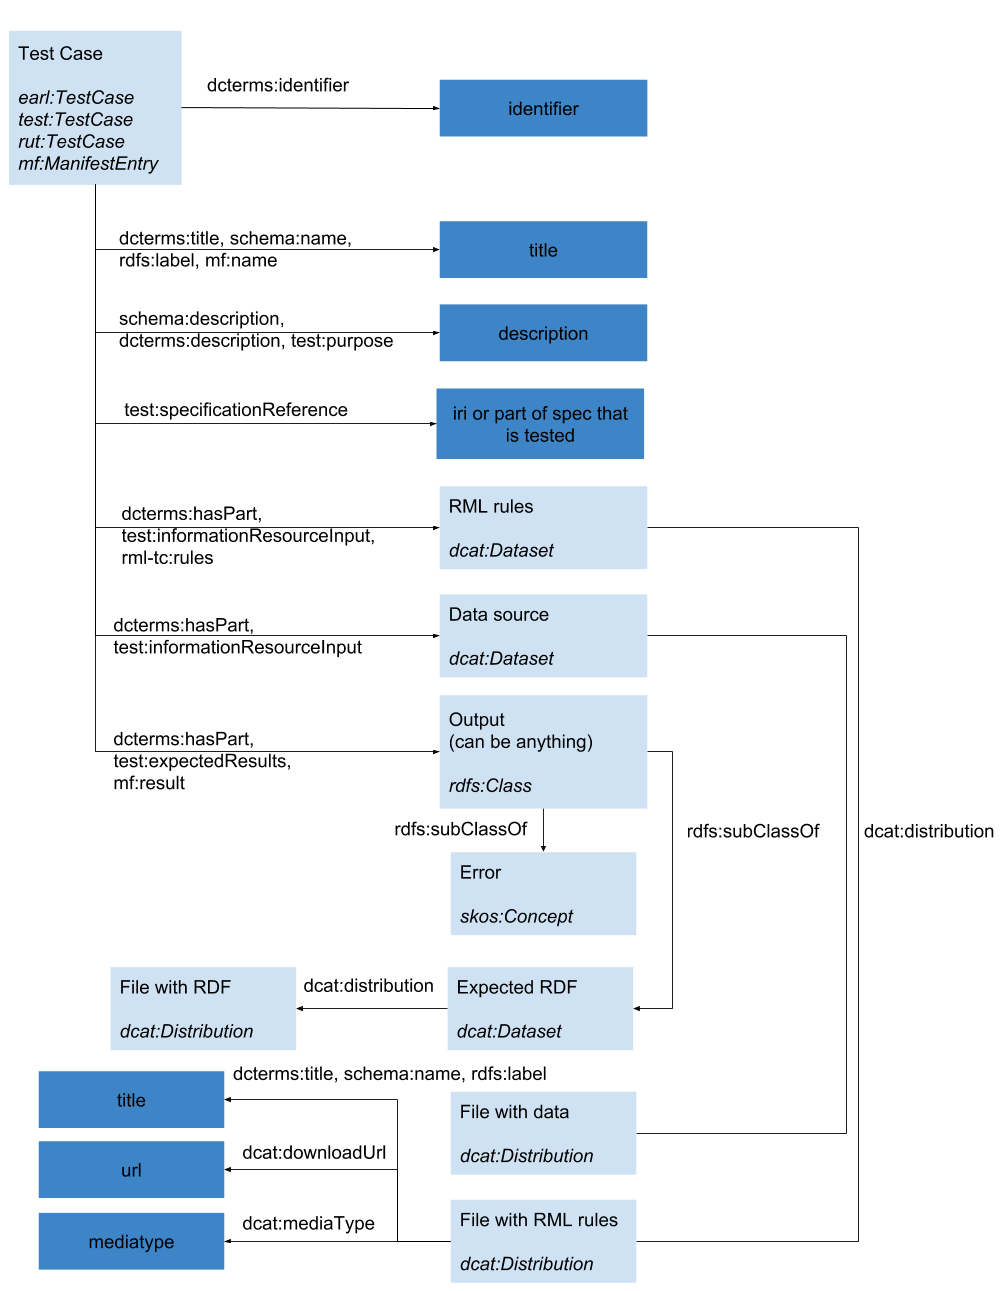
\includegraphics[width=0.9\textwidth]{figures/rml_test_case_model.png}
\caption{Data model of the RML test cases}
\label{fig:datamodel}
\end{figure}

We propose test cases to determine the conformance of RML processors to the RML specification. The proposed test cases are based on the R2RML test cases, but they take into account different heterogeneous data sources and the corresponding differences in RML. Our preliminary set of test cases includes (i)~adjusted R2RML test cases for relational databases (including MySQL\footnote{\url{https://www.mysql.com/}}, PostgreSQL\footnote{\url{https://www.postgresql.org/}}, and SQL Server\footnote{\url{https://www.microsoft.com/en-us/sql-server/}}) and (ii)~new test cases for files in the CSV, XML (with XPath as the reference formulation), and JSON format (with JSONPath as the reference formulation). The test cases are described at \url{http://rml.io/test-cases/} and the corresponding files are available at \url{https://github.com/rmlio/rml-test-cases}.

\subsubsection{Data model}

We describe the test cases semantically to increase their reusability and sharability. To this end, we created a semantic data model\footnote{\url{http://rml.io/test-cases/\#datamodel}}, with as main entity the test case (see Figure \ref{fig:datamodel}). For each test case, the following details are described: unique identifier, title, description, relevant aspect of the RML specification, data sources (optional), expected knowledge graph or error, and RML rules.

To provide the corresponding semantic descriptions, the model uses mostly the Evaluation and Report Language (EARL) 1.0 Schema\footnote{\url{https://www.w3.org/TR/EARL10/}, with prefix \texttt{earl}}, the Test case manifest vocabulary\footnote{\url{http://www.w3.org/2001/sw/DataAccess/tests/test-manifest\#}, with prefix \texttt{mf}}, the Test Metadata vocabulary\footnote{\url{https://www.w3.org/2006/03/test-description\#}, with prefix \texttt{test}}, and the Data Catalog Vocabulary\footnote{\url{https://www.w3.org/TR/vocab-dcat/}, with prefix \texttt{dcat}}. A test case is annotated with the classes \verb|earl:TestCase|, \verb|test:TestCase|, and \verb|mf:ManifestEntry|. The identifier, title, description, and the specific aspect of the RML specification that is being tested are added as datatype properties. The files that are provided as input to the tools are linked to the test cases via \verb|test:informationResourceInput| and \verb|dcterms:hasPart|. The file with the RML rules is also linked via \verb|rml-tc:rules|\footnote{\url{http://rml.io/ns/test-cases}, with prefix \texttt{rml-tc}}. The objects of these properties are of the class \verb|dcat:Dataset|,which in turn link to a \verb|dcat:Distribution| that includes a link to a file. The expected output, whether that is a knowledge graph or an error, is linked via \verb|test:expectedResults|, \verb|mf:result|, and \verb|dcterms:hasPart|. In the case of a knowledge graph, the object of these properties is a \verb|dcat:Dataset|, linked to a \verb|dcat:Distribution|, to describe the file containing the graph. In the case of an error, we link to the expected error.

\subsubsection{Test case files}

Each test case consists of a set of files that contain the input data sources, the RML rules, and the expected RDF output. In practice, the files are organized as follows: all files for a single test case are contained in a single folder. There are three types of files for each test case:

\begin{itemize}
  \item 0 or more \textbf{data source files} for CSV (with extension .csv), XML (with extension .xml), and SON (with extension .json), or 
  1 file with SQL statements to create the necessary tables for relational databases (called \verb|resource.sql|);
  \item 1 \textbf{file with the RML rules} (in Turtle format, called \verb|mapping.ttl|); and
  \item 0 or 1 \textbf{file with the expected RDF} (in N-Quads format, called \verb|output.nq|).
\end{itemize}

Distinct test cases assess different behaviors of the processors. Certain test cases assess the behavior of the tools when (i)~the required data sources are not available, and others when (ii)~an error occurs and no output is generated. In the former, no data sources files or SQL statements are provided. In the latter, no file with the expected RDF is provided. The test cases are independent of how the processors materialize the knowledge graph: a data dump, as done by the RMLMapper, or on the fly, as done by Ontario~\citep{endris2019ontario}.

\subsubsection{Differences with R2RML test cases}
For most R2RML test cases, we created an RML variant for CSV, XML, JSON, MySQL, PostgreSQL, and SQL Server, leading to 6 RML test cases per R2RML test case. For R2RML test cases that focus on specific features of SQL queries, we only created 3 RML test cases, i.e., for MySQL, PostgreSQL, and SQL Server.

For test cases with CSV, XML, and JSON files as data sources, we created the corresponding files with the data based on the tables of the relational databases. For CSV, we used the table created by the SQL statements of the R2RML test case and stored it as a CSV file. For XML, the name of the table was used for the root of the XML document and every row of the table was used to create an XML element. Within this element, elements were created for each column and their values are the values of the corresponding columns in the table. For JSON, we followed a similar approach as XML. The file contains a JSON object at the root with the name of the table as the only attribute. This attribute has as value an array, where each element of the array corresponds with a row in the table. For each row, attributes were created for each column and their values are the values of the corresponding columns in the table.

\paragraph{Data errors.}
2 of the R2RML test cases expect a data error to happen, e.g., when the subject IRI of an entity cannot be generated. In this case, an error is thrown and no knowledge graph is generated. With RML for entities where no subject IRI can be generated there is also no output generated, but, in contrast to R2RML, for the other entities the corresponding output is still generated. Therefore, for the corresponding RML test cases the processors can still throw an error, but the generation of the knowledge graph must not be halted.

\paragraph{Inverse expressions.}
3 of the R2RML test cases are designed to test the use of inverse expressions\footnote{\url{https://www.w3.org/TR/r2rml/\#inverse}}. However, inverse expressions are only used to optimize the knowledge graph generation and no differences are observed in the generated knowledge graph. Thus, whether inverse expressions are used by a processor or not cannot be verified by such test cases. Thus, we do not include them for RML.

\paragraph{SQL-specific features.}
18 of the R2RML test cases focus on specific features of SQL queries, e.g., a duplicate column name in a SELECT query. As there are no corresponding RML test cases for CSV files, XML files with XPath, and JSON files with JSONPath, we only provide 54 corresponding test cases for MySQL, PostgreSQL, and SQL Server.

\paragraph{Null values.}
1 of the R2RML test cases tests null values in the rows. However, a corresponding RML test case cannot be provided for the CSV and XML format, because both formats do not support null values.

\paragraph{Spaces in columns.}
1 of the R2RML test cases is designed to test the behaviour when dealing with spaces in the columns of the SQL tables. However, a corresponding RML test case cannot be provided for the XML format, because it does not allow spaces in names.
\\
\\
In total, we have 297 test cases: 39 for CSV, 38 for XML, 41 for JSON, and 180 for relational databases. Of these 297, 255 test cases expect an knowledge graph to be generated, while 36 expect an error that halts the generation.

\subsection{Conformance of RML Parsers}

In this section, we describe the executing of the test cases and their results for four RML processors: the RMLMapper, CARML, RocketRML and SDM-RDFizer. 
We detail on (i) the method for running the test cases and obtaining the results, which are annotated semantically, and (ii) the implementation report similar as proposed for R2RML\footnote{\url{https://www.w3.org/TR/rdb2rdf-implementations/}}. 

\subsubsection{Method}
We define a method to run the RML test cases over RML processors and generate the corresponding results. The main goal is to facilitate the testing process and provide a general solution for running the test cases over other RML processors that can be developed in the future. The method consists of two main steps: (i) assessing if a processor passes every test case and (ii) annotating the obtained results as RDF using the EARL Schema through a set of YARRRML rules~\citep{Heyvaert2018Declarative}.

We implemented a Java-based tool for checking the conformance of the test cases over different RML processors. At this moment, it is able to evaluate the test cases for JSON, CSV and XML formats. We relied on the test framework of each processor to execute the RDB test cases. If a new processor wants to be added to test its conformance, the framework only needs to have access to the corresponding output of each test-case. Then it checks, using the same method for all processors, if the output is the same as the correct one, if an error that is expected has really thrown, etc. It generates as output two CSV files with the results and the metadata needed to generate the corresponding RDF.

%For obtaining the RDF from the results 
The results are semantically annotated, as the test cases, using the EARL Schema. Each test case evaluated by a tool is annotated as an \texttt{earl:Assertion} with the properties: \texttt{earl:subject} with the URI of the tool, \texttt{earl:assertedBy} with the identifier of who performed the evaluation, \texttt{earl:test} with the URI of the test and \texttt{earl:result} with the result of the test-case. 

\begin{table}[]
\centering 
\caption[RML test-cases results for RMLMapper]{Results of the RMLMapper}
\label{tab:rmlmapper}
\begin{tabular}{c|c|c|c|c|c|c|c}

RMLMapper                 & \textbf{CSV} & \textbf{JSON} & \textbf{XML} & \textbf{MySQL} & \textbf{PostgreSQL} & \textbf{SQL Server} & \textbf{Total} \\ \hline
\textbf{passed}       & 39           & 41           & 38            & 55              & 55               & 55                   & 283             \\ \hline
\textbf{failed}       & 0           & 0           & 0            & 5              & 5                   & 5                   & 15             \\ \hline
\textbf{inapplicable} & 0            & 0             & 0             & 0             & 0                  & 0                  & 0            \\ 
\end{tabular}
\end{table}


\begin{table}[]
\centering
\caption{RML test-cases results for CARML}
\label{tab:carml}
\begin{tabular}{c|c|c|c|c|c|c|c}

CARML                 & \textbf{CSV} & \textbf{JSON} & \textbf{XML} & \textbf{MySQL} & \textbf{PostgreSQL} & \textbf{SQL Server} & \textbf{Total} \\ \hline
\textbf{passed}       & 29           & 28           & 28            & 0              & 0                   & 0                   & 85             \\ \hline
\textbf{failed}       & 10           & 10           & 13            & 0              & 0                   & 0                   & 33             \\ \hline
\textbf{inapplicable} & 0            & 0             & 0             & 60             & 60                  & 60                  & 180            \\ 
\end{tabular}
\end{table}


\begin{table}[]
\centering
\caption{RML test-cases results for RocketRML}
\label{tab:rocketrml}
\begin{tabular}{c|c|c|c|c|c|c|c}

RocketRML                & \textbf{CSV} & \textbf{JSON} & \textbf{XML} & \textbf{MySQL} & \textbf{PostgreSQL} & \textbf{SQL Server} & \textbf{Total} \\ \hline
\textbf{passed}       & 25           & 26          & 24            & 0              & 0                   & 0                   & 65             \\ \hline
\textbf{failed}       & 14           & 15           & 14            & 0              & 0                   & 0                   & 43             \\ \hline
\textbf{inapplicable} & 0            & 0             & 0             & 60             & 60                  & 60                  & 180            \\ 
\end{tabular}
\end{table}


\begin{table}[]
\centering
\caption{RML test-cases results for SDM-RDFizer}
\label{tab:sdm-rdfizer}
\begin{tabular}{c|c|c|c|c|c|c|c}

SDM-RDFizer                & \textbf{CSV} & \textbf{JSON} & \textbf{XML} & \textbf{MySQL} & \textbf{PostgreSQL} & \textbf{SQL Server} & \textbf{Total} \\ \hline
\textbf{passed}       & 39           & 41           & 38            & 60              & 60                   & 60                   & 298             \\ \hline
\textbf{failed}       & 0           & 0           & 0            & 0              & 0                   & 0                   & 0             \\ \hline
\textbf{inapplicable} & 0            & 0             & 0             & 0             & 0                  & 0                  & 0            \\ 
\end{tabular}
\end{table}


Three types of results are possible: ``passed'', ``failed'', and ``inapplicable''.The option \textbf{Passed} (\texttt{earl:passed}) is used either when the actual output matches the expected output when no error is expected, or when the tool throws an error when an error is expected. \textbf{Failed} (\texttt{earl:failed}) is used either when the actual output does not match the expected output if no error is expected, the processor returns an error trying to execute a test or the tool does not throw error if an error is expected. \textbf{Inapplicable} (\texttt{earl:inapplicable}) is used when the tool clearly states that specific features used in a test case are not supported. The results also provide its type (\texttt{earl:TestResult}) and its mode (\texttt{earl:automatic} for all these cases). 
We created a set of YARRRML rules to generate these annotations following the EARL Schema that, using the outputs of the test cases.

\subsubsection{Results}
We perform the test-cases over four processors. In Table \ref{tab:rmlmapper} we show the results for the RMLMapper processor. It passes all CSV, JSON and XML test cases, but fails in the same 5 test cases for the RDBs. The failures are related to the automatic datatyping of literal for RDBs specified by R2RML\footnote{\url{https://www.w3.org/TR/r2rml/\#dfn-natural-rdf-literal}}. RMLMapper expects to pass the failed test-cases in next versions of the processor. The effort prediction to pass these test-cases is not very much since the failures depend on the general processor, not on the used RDBMS. Once they have been solved for one RDBMS they will automatically pass over the rest.

In Table \ref{tab:carml} we show the results for the CARML processor. It partially passes the CSV, JSON and XML test cases, but it does not provide support for any of the RDBs test cases. The failures are related to the unsupported for multiple Subject Maps, multiple Predicate Maps, and Named Graphs. The developers of the tool declare that CARML will support these features in next versions of the processor. However, at the moment of writing, we do not have any information about if CARML will provide support for RDBs.

Table \ref{tab:rocketrml} shows the results for the RocketRML processor. Its behavior is similar to CARML, as it partially passes the CSV, JSON and XML test cases, but it does not provide support for any of the RDBs test cases. Finally, Table \ref{tab:sdm-rdfizer} show the results for the SDM-RDFizer processor, which passes all the proposed test cases, having a similar behavior as the RMLMapper engine.

Finally, we can declare that testing a RML processor with the defined cases and analyzing the obtained results offers a general view of the current status of it. These results also give useful information to the tool developers on knowing where they should put their effort to improve the conformance of the processor.

